\chapter{System architecture}
\label{sec:architecture}

Figure~\ref{fig:pipeline} shows the pipeline. A question passes through five stages; each stage can stop the run
with an explicit status instead of producing a doubtful answer: \emph{referred} (a ruling question, sent to scholars),
\emph{unanswered} (no sentence could be supported by the sources), or \emph{signed}.

\begin{figure}[ht]
\centering
\resizebox{\textwidth}{!}{%
\begin{tikzpicture}[
  node distance=6mm and 7mm,
  box/.style={draw=navy, rounded corners=2pt, fill=soft, align=center, font=\small, minimum height=11mm,
              text width=27mm, inner sep=3pt},
  data/.style={draw=gray!60, fill=white, align=center, font=\scriptsize, text width=27mm, inner sep=2pt,
               shape=rectangle, rounded corners=1pt},
  stop/.style={draw=amberx!90!black, fill=amberx!12, align=center, font=\scriptsize, text width=22mm, rounded corners=2pt},
  arr/.style={-{Stealth[length=2mm]}, thick, navy},
  dsh/.style={-{Stealth[length=1.6mm]}, gray!70, dashed}]
  \node[box] (q) {\textbf{Question}\\EN / AR (TR, UR)};
  \node[box, right=of q] (g) {\textbf{1. Ruling pre-check}\\regex + content levels};
  \node[box, right=of g] (r) {\textbf{2. Hybrid retrieval}\\BM25 $\oplus$ E5 (RRF)};
  \node[box, right=of r] (a) {\textbf{3. Grounded answer}\\LLM + support check};
  \node[box, below=16mm of a] (gl) {\textbf{4. Glossing}\\LLM restricted\\to lexicon glosses};
  \node[box, left=11mm of gl] (p) {\textbf{5. Pose assembly}\\sign lookup, proportions,\\transitions};
  \node[box, left=of p] (sk) {\textbf{Skeleton video}\\MP4, 25 fps};
  \node[box, left=of sk] (av) {\textbf{3D avatar}\\VRM, outfits, speed,\\export};
  \node[data, above=4mm of r] (kb) {Qur'an (6,236 verses) + HadeethEnc hadith; e5-large index};
  \node[data, below=5mm of gl] (lex) {Sign lexicons: ASL 3,055 / ArSL 3,979 glosses};
  \node[data, below=5mm of p] (bt) {Back-translation: DTW 1-NN recogniser $\rightarrow$ gloss accuracy, WER};
  \node[stop, above=4mm of g] (ref) {\emph{referred}\\to scholars};
  \node[stop, above=4mm of a] (un) {\emph{unanswered}\\(no supported sentence)};
  \draw[arr] (q) -- (g); \draw[arr] (g) -- (r); \draw[arr] (r) -- (a);
  \draw[arr] (a) -- node[right, font=\scriptsize, text width=24mm]{answer + citations} (gl);
  \draw[arr] (gl) -- node[above=1pt, font=\scriptsize, fill=white, inner sep=1pt]{glosses} (p);
  \draw[arr] (p) -- (sk); \draw[arr] (p.north west) to[bend right=22] node[above, font=\scriptsize]{pose} (av.north east);
  \draw[dsh] (kb) -- (r); \draw[dsh] (lex) -- (gl); \draw[dsh] (lex.west) -- (p.south east);
  \draw[dsh] (p) -- (bt);
  \draw[dsh] (g) -- (ref); \draw[dsh] (a) -- (un);
\end{tikzpicture}}
\caption{The Isharati pipeline. Solid arrows: the signing path. Dashed: data each stage reads, the two exits that
stop a run without signing, and the back-translation check of the generated pose.}
\label{fig:pipeline}
\end{figure}

\paragraph{Stage 1: ruling pre-check.} Before any language-model call, a per-language pattern list (for example
\emph{halal, haram, fatwa, permissible, ``can I''} in English; \ar{حلال، حرام، يجوز} in Arabic; \emph{helal, caiz, fetva}
in Turkish; \ar{جائز، فتوی} in Urdu) and for Arabic, the content-level guard of the earlier Arabic lesson application (levels C,
disputed matters, and D, rulings) refer the question to a scholar. The patterns favour caution: the Arabic
term \ar{حكم} also matches \ar{حكمة} (wisdom), so such questions are referred too. The system never issues a ruling.

\paragraph{Stage 2: hybrid retrieval.} The language model adds up to 14 search keywords to the question. BM25
\cite{bm25} ranks passages for the question plus keywords and dense retrieval with multilingual E5 \cite{me5} ranks them for the
question as asked; the two rankings (top 100 each) are fused by reciprocal rank fusion \cite{rrf}, and the top 10
passages go to the answering step (Chapter~\ref{sec:knowledge}).

\paragraph{Stage 3: grounded answer.} The model picks the most direct passage, writes two to four sentences that cite
passages by number, and every sentence is checked against the passages it cites. Unsupported sentences are dropped and
reported; if fewer than two sentences survive, the model rewrites once (Section~\ref{sec:grounding}).

\paragraph{Stage 4: glossing (Generative AI translation).} The answer produced by the LLM is turned into a gloss sequence. To ensure correct signing, the LLM is restricted to using only available lexicon glosses, assisted by robust morphological analysis (for example, mapping inflected forms like "loving" back to the root "love"). Words without an available sign are reported (Section~\ref{sec:glossing}).

\paragraph{Stage 5: pose assembly and rendering.} Each gloss is replaced by its recorded sign; body proportions are
normalised across sources and smooth transitions are inserted; the pose is rendered as a skeleton video and drives the
3D avatar in the browser (Section~\ref{sec:render}). Every run writes a report (answer, sources, glosses, missing signs,
coverage, per-word trace, back-translation score) next to the video.

\section{Core operational capabilities}
\label{sec:modes}
Isharati provides three distinct functional modes designed for different user workflows, ranging from generative conversational inquiry to direct scriptural study:

\subsection{Mode 1: Grounded Retrieval-Augmented Generation (Grounded Q\&A)}
\label{sec:mode_rag}
The primary conversational mode enables users to ask open-ended questions about Islamic principles, worship, and ethics. To prevent theological hallucinations, the pipeline operates under strict retrieval-augmented constraints:
\begin{enumerate}[leftmargin=*,itemsep=2pt]
  \item \textbf{Dense embedding space:} We employ \code{intfloat/multilingual-e5-large} \cite{me5}, a 1,024-dimensional multilingual transformer. Passages are indexed with the prefix \code{"passage: "} and questions with \code{"query: "}. All vectors are $L_2$-normalized, mapping queries and scripture into a shared metric space where semantic proximity corresponds directly to cosine similarity.
  \item \textbf{Corpus vector index:} The retrieval index spans the entire canonical Qur'an (6,236 verses in Uthmani script) and authenticated hadith collections from HadeethEnc (3,574 Arabic, 2,328 English, 2,150 Turkish, and 2,220 Urdu passages).
  \item \textbf{Hybrid retrieval fusion:} Query execution combines dense vector search with sparse BM25 lexical ranking \cite{bm25}. The language model first enriches the query by generating up to 14 domain-specific theological keywords. BM25 scores the expanded keyword query, while dense retrieval scores the original natural-language query. The top-100 candidates from each method are merged using Reciprocal Rank Fusion (RRF, smoothing constant $k{=}60$) \cite{rrf}:
  \begin{equation}
    \mathrm{RRF\_Score}(d) = \frac{1}{60 + r_{\text{dense}}(d)} + \frac{1}{60 + r_{\text{sparse}}(d)}.
  \end{equation}
  The top-10 reranked passages are passed to the answering model.
  \item \textbf{Constrained generative answering and verification:} An instruction-tuned LLM (Qwen 2.5 72B / Nemotron-3 Super 120B) is prompted to write a concise 2--4 sentence answer citing passages strictly by index. Crucially, an automated post-generation support verifier checks every sentence against the text of its cited passages. If a sentence introduces ungrounded claims, it is discarded. If fewer than two supported sentences survive, the query triggers the \emph{unanswered} status.
  \item \textbf{Ruling pre-check guard:} Jurisprudential ruling queries (*fatwa*, *halal*, *haram*, \ar{حكم، يجوز}) are intercepted by deterministic regexes and routed directly to the \emph{referred} status, ensuring the system never fabricates religious rulings.
\end{enumerate}

\subsection{Mode 2: Morphological analysis and pose concatenation (Studio mode)}
\label{sec:mode_studio}
For educators, content creators, and translators who need to synthesize arbitrary signed text without generative rewriting, Isharati provides a direct \emph{Studio} mode. The input text is translated into sign glosses via deep morphological analysis and assembled into a continuous 3D performance.

\paragraph{Morphological analysis pipeline.} Raw natural language cannot be mapped word-for-word to sign lexicons due to clitics, affixes, and inflection. The morphological subsystem executes language-specific decomposition:
\begin{itemize}[leftmargin=*,itemsep=2pt]
  \item \textbf{Arabic morphology (CAMeL Tools):} Arabic words are heavily agglutinative. The pipeline applies orthographic normalization, strips conjunction proclitics (\ar{و، ف}), prepositional clitics (\ar{ب، ك، ل}), and the definite article (\ar{ال}), followed by possessive pronominal enclitics (\ar{هم، نا، ك، ي}). CAMeL Tools \cite{camel} resolves the underlying root and dictionary lemma. Semantic collision guards prevent false positives (e.g., guaranteeing that \ar{إسلام} never conflates with \ar{سلام} [peace], nor \ar{شرك} [polytheism] with \ar{شر} [evil]). Multi-word phrase signs (\ar{محمد رسول الله}, \ar{الله أكبر}) are prioritized as atomic lexical units.
  \item \textbf{English morphology:} Words are normalized for case and punctuation, possessives are removed, and inflectional morphology is reduced to base stems (e.g., mapping \emph{loving} $\rightarrow$ \emph{love}, \emph{believers} $\rightarrow$ \emph{believer}, and \emph{prayed} $\rightarrow$ \emph{pray}).
\end{itemize}

\paragraph{Walkthrough of an example prompt.} To illustrate, consider the complex Arabic input prompt:
\begin{center}
\ar{\textbf{«وبالصلوات المفروضة يتقرب المؤمنون»}}\\
\textit{(``And with the obligatory prayers, the believers draw near'')}
\end{center}
The morphological decomposition and gloss matching proceed as follows:
\begin{enumerate}[leftmargin=*,itemsep=1pt]
  \item \textbf{Token 1: \ar{«وبالصلوات»}}
    \begin{itemize}[leftmargin=*,itemsep=0pt]
      \item \textit{Clitic stripping:} Conjunction \ar{و} (and) + preposition \ar{ب} (with) + article \ar{ال} (the) stripped $\rightarrow$ stem \ar{صلوات}.
      \item \textit{Morphological lemmatization:} CAMeL Tools identifies broken/sound plural feminine form and maps to lemma \ar{صلاة}.
      \item \textit{Lexicon lookup:} Exact match with ArSL gloss \ar{الصلاة} (\textsc{Prayer}).
    \end{itemize}
  \item \textbf{Token 2: \ar{«المفروضة»}}
    \begin{itemize}[leftmargin=*,itemsep=0pt]
      \item \textit{Clitic stripping:} Article \ar{ال} stripped $\rightarrow$ feminine adjective stem \ar{مفروضة}.
      \item \textit{Morphological lemmatization:} Maps to lemma \ar{فرض}.
      \item \textit{Lexicon lookup:} Matches ArSL gloss \ar{فرض} (\textsc{Obligatory}).
    \end{itemize}
  \item \textbf{Token 3: \ar{«يتقرب»}}
    \begin{itemize}[leftmargin=*,itemsep=0pt]
      \item \textit{Clitic stripping:} None. Imperfect verb prefix \ar{يـ} analyzed.
      \item \textit{Morphological lemmatization:} Verb Form V lemma mapped to root \ar{قرب}.
      \item \textit{Lexicon lookup:} Matches ArSL gloss \ar{قريب} (\textsc{Near}).
    \end{itemize}
  \item \textbf{Token 4: \ar{«المؤمنون»}}
    \begin{itemize}[leftmargin=*,itemsep=0pt]
      \item \textit{Clitic stripping:} Article \ar{ال} + masculine plural suffix \ar{ـون} stripped $\rightarrow$ stem \ar{مؤمن}.
      \item \textit{Morphological lemmatization:} Maps to lemma \ar{مؤمن}.
      \item \textit{Lexicon lookup:} Matches ArSL gloss \ar{مؤمن} (\textsc{Believer}).
    \end{itemize}
\end{enumerate}
The resulting gloss sequence is \ar{[الصلاة، فرض، قريب، مؤمن]} (\textsc{[Prayer, Obligatory, Near, Believer]}). Any word lacking a corresponding recording in the active lexicon is flagged in red in the UI trace and assigned a 12-frame pause/hold rather than incorrect fingerspelling.

\paragraph{Kinematic pose concatenation.} The poser retrieves the preprocessed 3D joint coordinate arrays for each resolved gloss:
\begin{itemize}[leftmargin=*,itemsep=1pt]
  \item \textbf{Proportional rescaling:} Head-to-neck height is rescaled about the neck joint to a standard 0.74 shoulder-width ratio, eliminating scale discrepancies between signers.
  \item \textbf{Smoothstep interpolation:} Consecutive sign clips are spliced using an 8-frame cubic Hermite smoothstep curve ($S(t) = 3t^2 - 2t^3$), preventing unnatural snapping of wrists and hands.
  \item \textbf{Rest buffering:} A 5-frame lead-in and 15-frame lead-out buffer return the avatar smoothly to a resting pose.
\end{itemize}

\subsection{Mode 3: Authoritative scriptural retrieval (Qur'an recitation and Tafsir dashboard)}
\label{sec:mode_quran}
The third operational mode provides zero-hallucination, structured access to official signed performances of the Holy Qur'an and its authoritative interpretations. Rather than passing through generative LLMs, this module performs deterministic database lookups over pre-indexed, authenticated datasets:
\begin{enumerate}[leftmargin=*,itemsep=2pt]
  \item \textbf{Three authoritative signed sources:}
    \begin{itemize}[leftmargin=*,itemsep=1pt]
      \item \textbf{King Fahd Complex (KFC):} Authoritative signed explanations (*Tafsir*) produced by the King Fahd Complex for the Printing of the Holy Qur'an in Madinah.
      \item \textbf{Al-Mukhtasar fi Tafsir:} Simplified, accessible signed interpretations covering the meanings of Qur'anic passages.
      \item \textbf{Al-Kharj Education Department Curriculum:} Complete signed recitation of 22 short Surahs, synchronized word-by-word with the canonical audio recitation.
    \end{itemize}
  \item \textbf{API data contract and navigation:}
    \begin{itemize}[leftmargin=*,itemsep=1pt]
      \item \code{GET /api/quran/coverage}: Evaluates all 114 Surahs and returns coverage classification per Surah (\code{"both"}, \code{"recitation"}, \code{"tafsir"}, or \code{"none"}).
      \item \code{GET /api/quran/ayah?surah=N\&ayah=M}: Directly queries the verse index, returning metadata, Whisper-aligned word timestamps, Uthmani verse text, Tafsir transcriptions, and a fallback pointer to the nearest covered verse (\code{nearest: [surah, ayah]}) for uncovered ayahs.
      \item \code{GET /api/quran/pose/\{source\}/\{segment\_id\}.json}: Delivers pre-extracted continuous 3D MediaPipe pose frames.
    \end{itemize}
  \item \textbf{Dual-view interactive player:} The dashboard embeds the official source video alongside the synchronized 3D avatar / skeleton renderer, allowing viewers to verify avatar accuracy against the human signer frame by frame.
\end{enumerate}

\paragraph{Implementation.} Python 3 (FastAPI server, NumPy), MediaPipe Holistic for keypoints, CAMeL Tools
\cite{camel} for Arabic morphology, \code{intfloat/multilingual-e5-large} served locally for embeddings, and an LLM chain
of NVIDIA NIM models \cite{nvidianim} (Nemotron-3 Super 120B, then Nemotron-3 Ultra 550B, 25\,s timeout each) with
Groq's \code{gpt-oss-120b} as the last fallback. The avatar is rendered with three.js \cite{threejs} and three-vrm
\cite{threevrm}. The test suite has 194 passing tests.

\begin{figure}[ht]
\centering
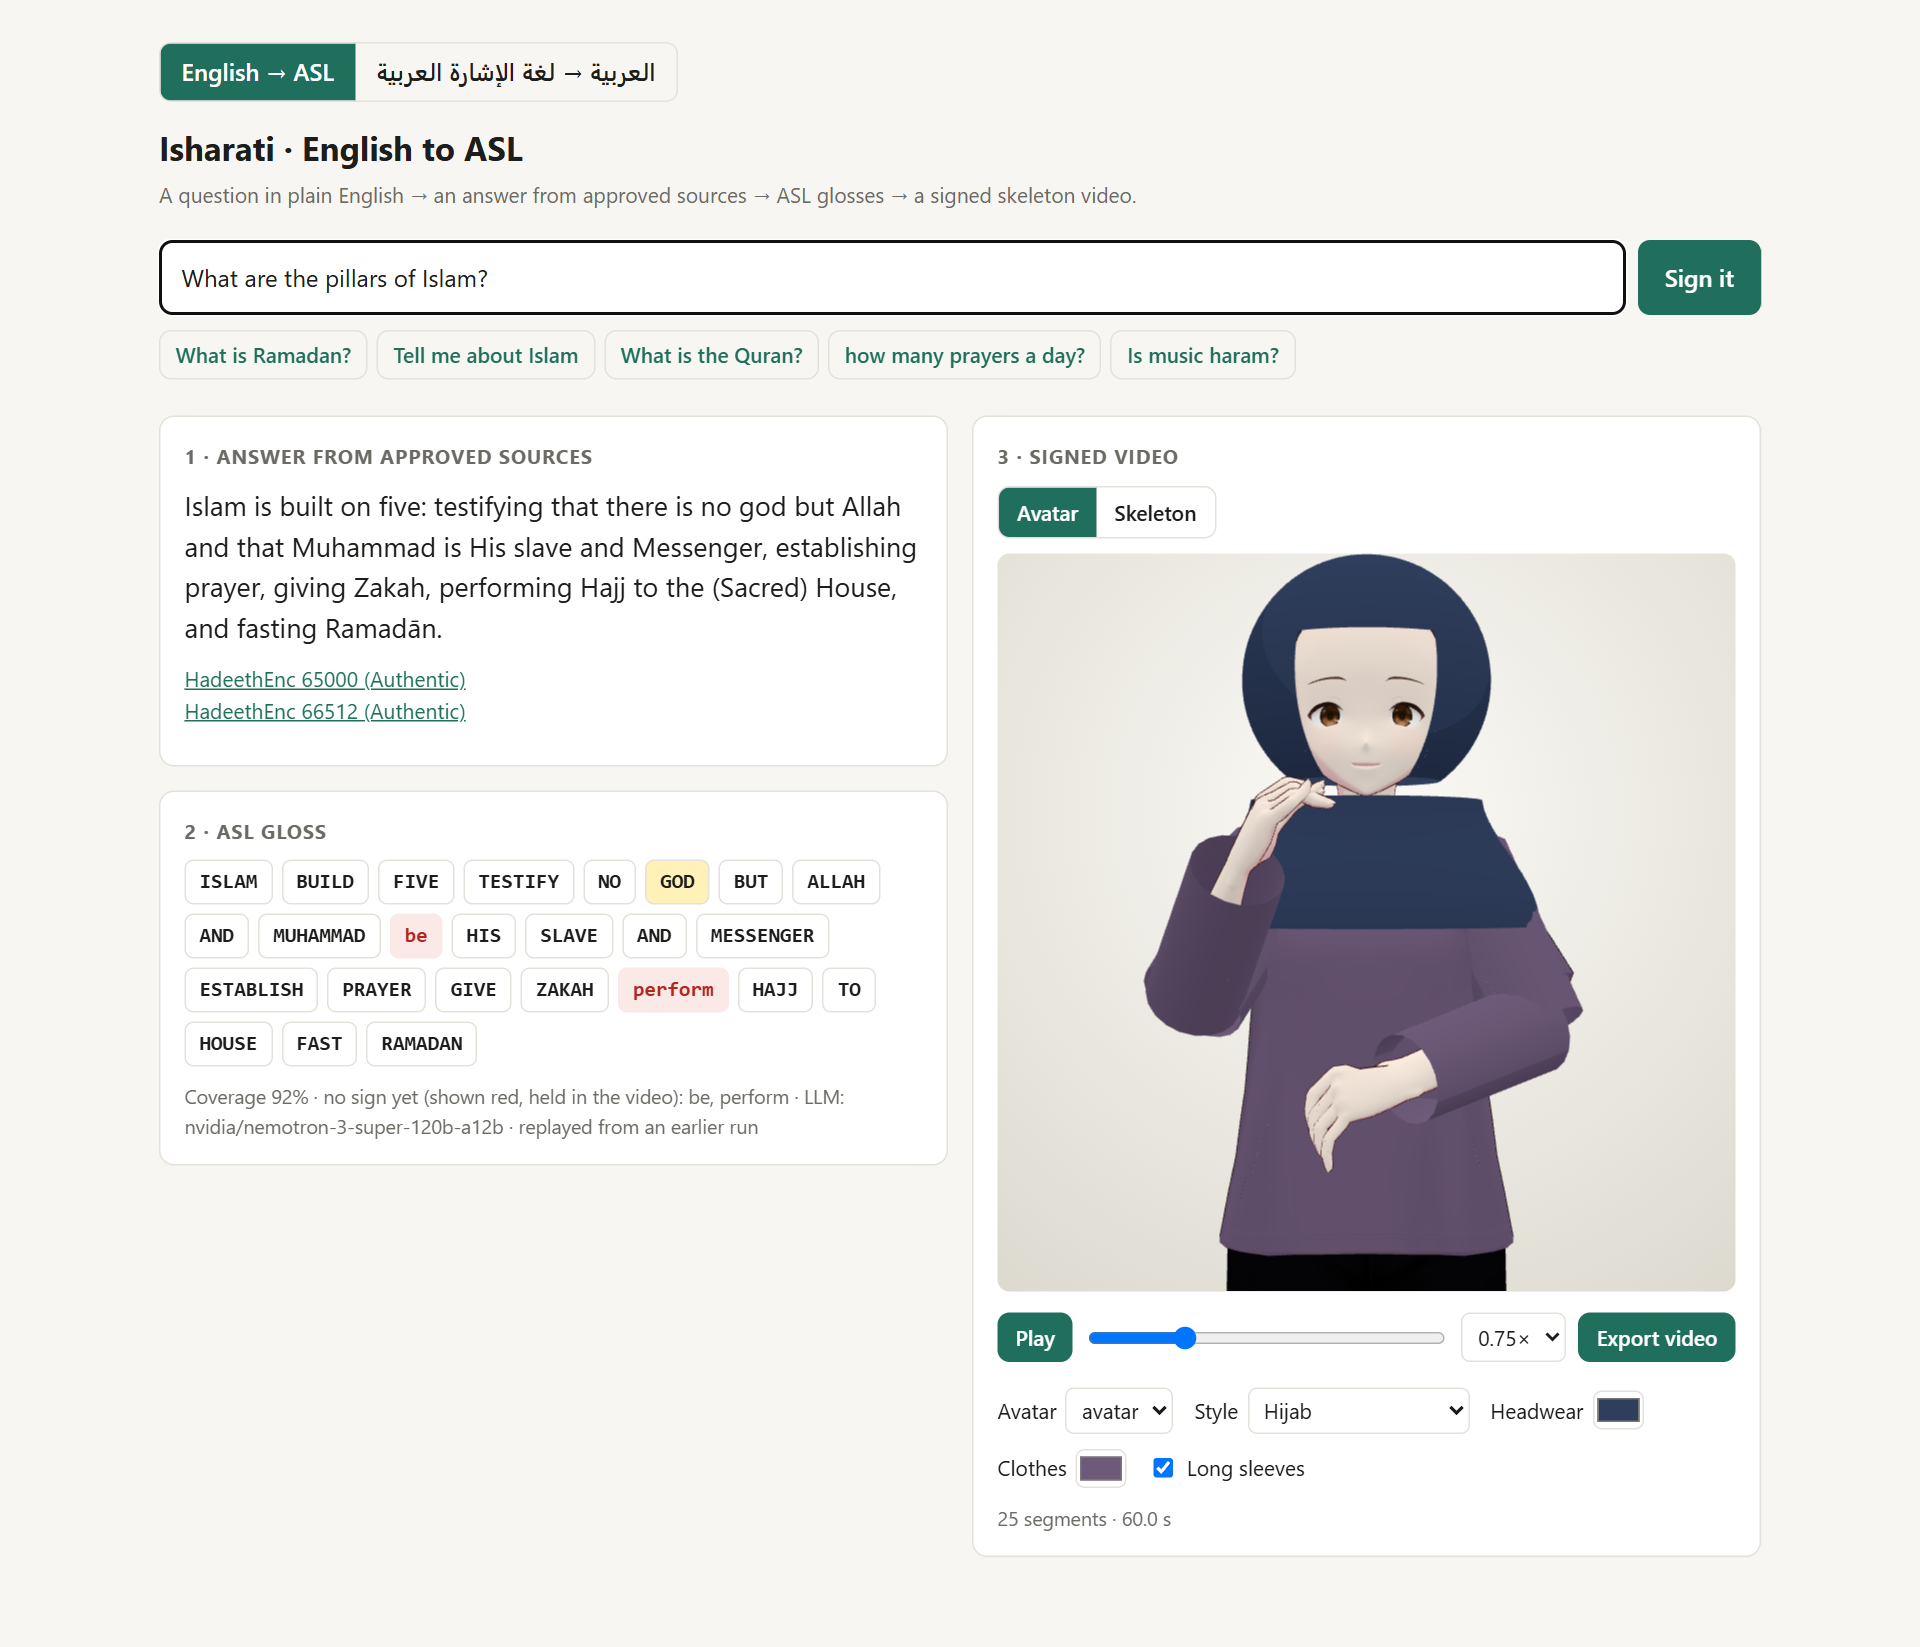
\includegraphics[width=0.49\textwidth]{figures/ui_en.png}\hfill
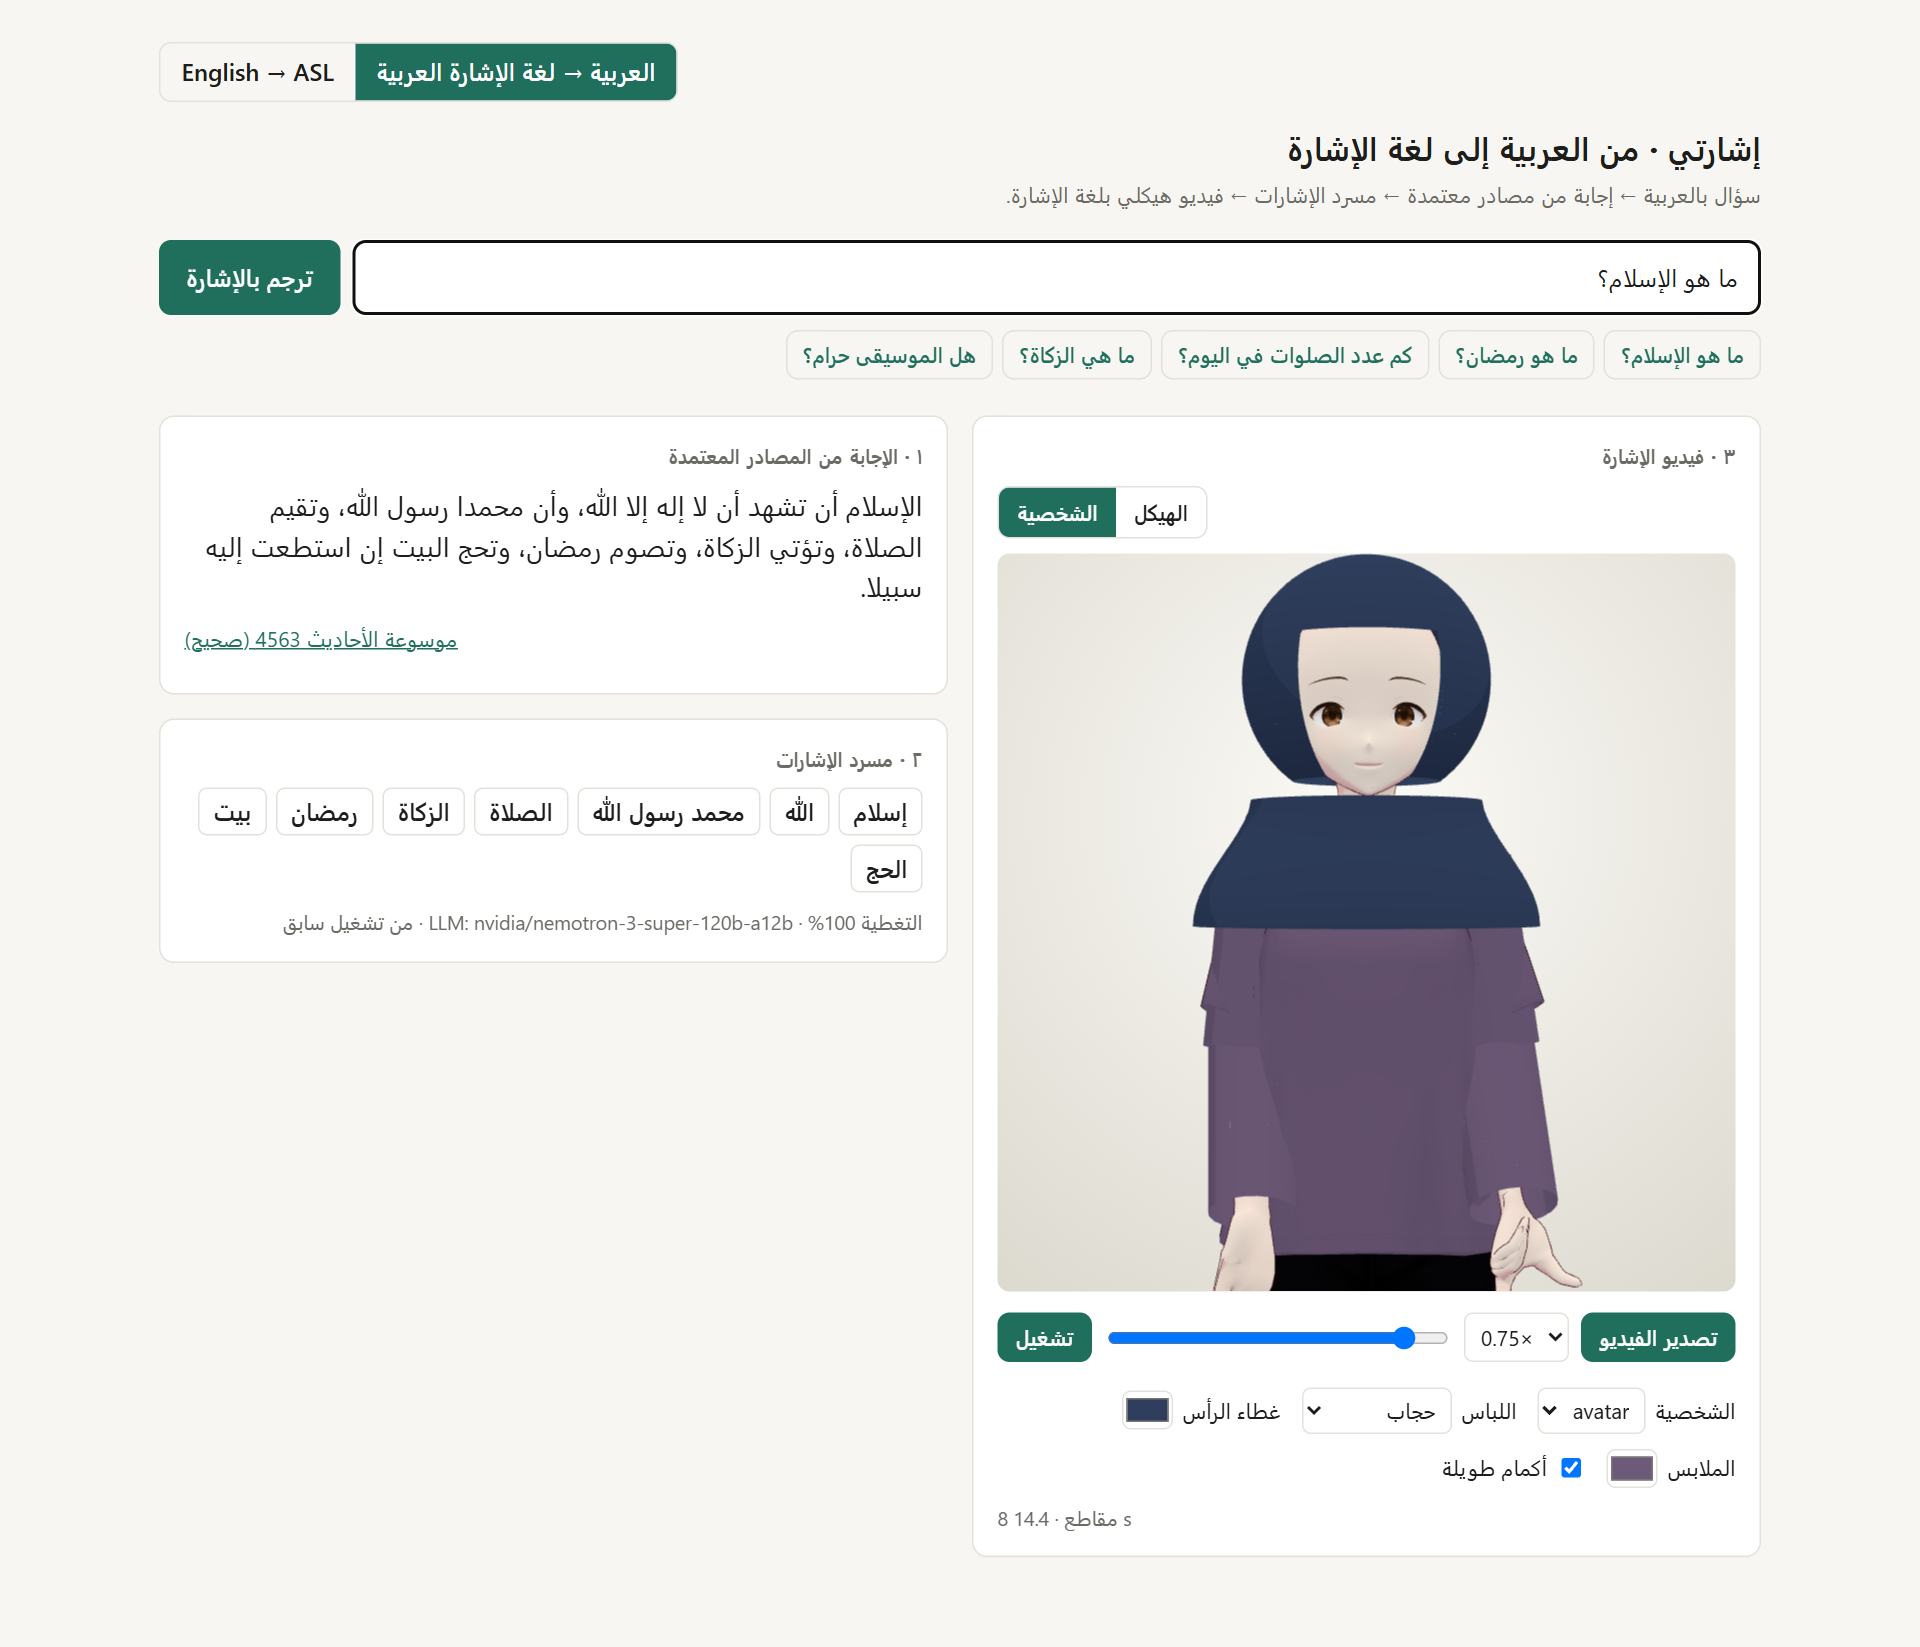
\includegraphics[width=0.49\textwidth]{figures/ui_ar.png}
\caption{The web application answering ``What are the pillars of Islam?'' in
English/ASL (left) and \ar{ما هو الإسلام؟} in Arabic/ArSL (right): grounded answer with its source links, the gloss
sequence (highlighted while signing), the avatar with the outfit panel, and the speed selector.}
\label{fig:ui}
\end{figure}
